\section{Travail effectue}
    À mon arrivée chez \emph{mediarithmics}, il a été décidé que mon sujet porterait sur l'optimisation de \emph{bid}. 
    Ainsi, dans cette partie je vais dans un premier temps présenter qu'est ce que le \emph{Real-Time Bidding} et les 
    objectifs d'un \emph{bid optimizer}. Dans un second temps, je présenterai l'analyse de la solution existante chez 
    \emph{mediarithmics} pour répondre à ce problème. Dans une troisième partie je dresserai une présentation de la 
    veille technologique effectuée autour de cette problématique. Ensuite, j'aborderai l'implémentation de la solution 
    ainsi que son suivi en production. Enfin, j'évoquerai les pistes d'amélioration autour du travail réalisé.
    \subsection{Online Bid Optimization} 
        \subsubsection{Presentation du Real-Time Bidding}
            Avant d'aborder, le sujet du \emph{bid optimizer}, il faut premièrement expliquer ce qu'est le 
            \emph{real-time bidding}. En temps réel, lorsque un internaute charge une page, avec des emplacements 
            publicitaires, ces derniers sont mis aux enchères auprès d'un \emph{Adexchange}. Un \emph{Adexchange} est 
            une plateforme automatisée d'achat et de vente en ligne et en temps réel. Elle permet donc à des 
            \emph{annonceurs}\footnote{acteurs cherchant à diffuser des publicités et achetant les emplacements} 
            et à des \emph{publishers}\footnote{acteurs affichant et vendant des emplacements} d'interragir. Prenons
            un exemple. Un \emph{publisher} possède un site internet sur lequel il a défini des emplacements 
            publicitaires. Le publisher a référencé ces emplacement auprès d'un  \emph{Adexchange}. De leurs côtés des 
            annonceurs ont indiqués à l'Adexchange leur volonté d'afficher de la publicité à des internautes. Ainsi,
            lorsque un utilisateur va venir charger une page web du site du publisher contenant un emplacement 
            publicitaire référencé, une requête est envoyée à l'Adexchange avec toutes les données disponibles sur 
            l'utilisateur ainsi que des informations contextuelles, telles que l'\emph{id} de l'emplacement ou encore 
            celui du site web. L'Adexchange va alors informer tous les annonceurs qu'un emplacement publicitaire est 
            disponible et l'enchère est ouverte. Connaissant les informations de l'utilisateur ainsi que les données 
            contextuelles, les annonceurs vont alors placer une enchère. L'annonceur ayant l'emchère la plus haute est 
            alors informé par l'Adexchange qui demande à l'annonceur gagnant quel publicité ce dernier veut afficher.
            À la vue de cet exemple, il apparaît une difficulté majeure pour les annonceurs, quelle enchère placer. En 
            effet en fonction de la campagne publicitaire, des informations sur l'emplacement publicitaire ainsi que 
            sur l'utilisateur, il convient de définir un prix d'achat. Il apparaît clairement la nécessité de 
            recquerir à un système d'optimisation d'enchères.
            \begin{figure}
                \centering
                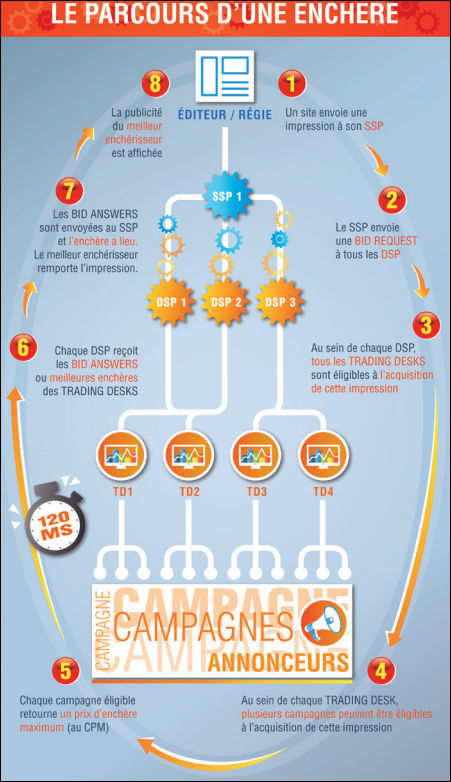
\includegraphics[scale=0.3]{images/rtb.jpg}
                \caption{Schmématisation du \textbf{RTB} \url{https://www.definitions-marketing.com/wp-content/uploads/2016/04/rtb.jpg}}
            \end{figure}
        \subsubsection{Objectifs d'un bid optimizer}
            \begin{figure}
                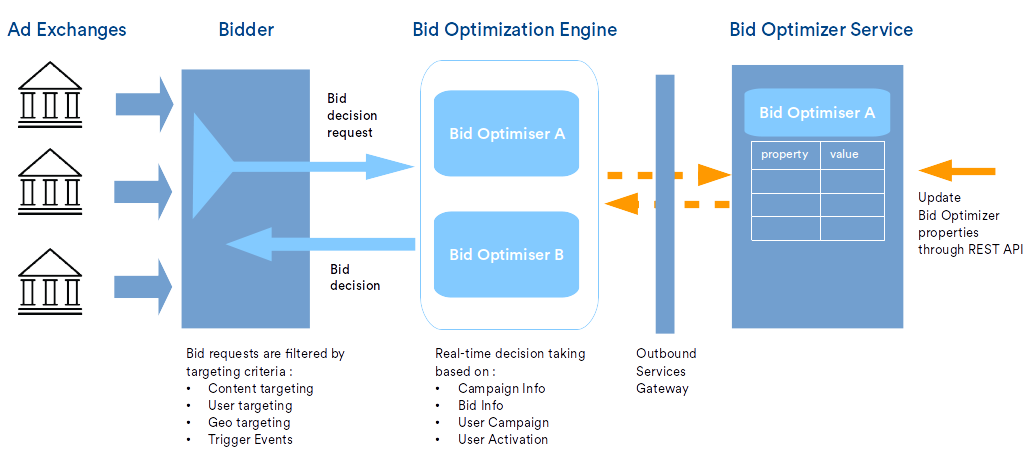
\includegraphics[width=\linewidth]{images/bid-optimization-engine-and-bid-optimizer.png}
                \caption{Schéma du concept de \textbf{bid optimizer} chez \emph{mediarithmics}}
                \label{fig:bid-optimization}
            \end{figure}
    \subsection{Analyses de la solution existante}
        \subsubsection{Diagnostic}
        \subsubsection{Axes d'amelioration}
        \subsubsection{Definition des problematiques et contours du probleme}
    \subsection{Veille technologique}
    \subsection{Implementation de la solution}
    \subsection{Suivi en production}
    \subsubsection{Pistes d'ameliorations et POC}        
